%----------------------------------------------------------------------------------------
%	PACKAGES AND OTHER DOCUMENT CONFIGURATIONS
%----------------------------------------------------------------------------------------

\documentclass[twoside,twocolumn]{article}
%________My packages Begin_____________________________________

\usepackage{graphicx} % for figures
\usepackage{float}% necessary "begin{figure}[H] to Place the float at precisely the location in the LaTeX code.
%=--------------------Francais------------
\usepackage[french]{babel} %Texte en fran�ais
\usepackage{lmodern}
\usepackage[utf8]{inputenc}
%-------------------------------

\usepackage[normalem]{ulem}
\usepackage{mathtools}
\usepackage{fourier}
\usepackage{enumitem}
\usepackage[skins,theorems]{tcolorbox}% for boxing and coloring equations
\usepackage{amsmath,amsthm,amssymb}
%-----
\apptocmd{\thebibliography}{\csname phantomsection\endcsname\addcontentsline{toc}{chapter}{\bibname}}{}{}
\usepackage[toc,page]{appendix}
\usepackage[nottoc]{tocbibind}
%\usepackage{lmodern}
%\renewcommand{\familydefault}{lmodern}
\usepackage{stfloats}
\usepackage{amsmath}

%________My packages End _________________________

%\usepackage[sc]{mathpazo} % Use the Palatino font

\usepackage[T1]{fontenc} % Use 8-bit encoding that has 256 glyphs
\linespread{1.05} % Line spacing - Palatino needs more space between lines
\usepackage{microtype} % Slightly tweak font spacing for aesthetics

%\usepackage[english]{babel} % Language hyphenation and typographical rules

\usepackage[hmarginratio=1:1,top=28mm,columnsep=30pt]{geometry} % Document margins
\usepackage[hang, small,labelfont=bf,up,textfont=it,up]{caption} % Custom captions under/above floats in tables or figures
\usepackage{booktabs} % Horizontal rules in tables

\usepackage{lettrine} % The lettrine is the first enlarged letter at the beginning of the text

\usepackage{enumitem} % Customized lists
\setlist[itemize]{noitemsep} % Make itemize lists more compact

\usepackage{abstract} % Allows abstract customization
\renewcommand{\abstractnamefont}{\normalfont\bfseries} % Set the "Abstract" text to bold
\renewcommand{\abstracttextfont}{\normalfont\small\itshape} % Set the abstract itself to small italic text

\usepackage{titlesec} % Allows customization of titles
\renewcommand\thesection{\Roman{section}} % Roman numerals for the sections
\renewcommand\thesubsection{\roman{subsection}} % roman numerals for subsections
\titleformat{\section}[block]{\large\scshape\centering}{\thesection.}{1em}{} % Change the look of the section titles
\titleformat{\subsection}[block]{\large}{\thesubsection.}{1em}{} % Change the look of the section titles

\usepackage{fancyhdr} % Headers and footers
\pagestyle{fancy} % All pages have headers and footers
\fancyhead{} % Blank out the default header
\fancyfoot{} % Blank out the default footer
\fancyhead[C]{Identification et Filtrage (IDFIL) : Travaux Pratiques n° 1 $\bullet$ Ecole Centrale de Nantes $\bullet$} % Custom header text
\fancyfoot[RO,LE]{\thepage} % Custom footer text

\usepackage{titling} % Customizing the title section

\usepackage[hidelinks]{hyperref} % For hyperlinks in the PDF

%----------------------------------------------------------------------------------------
%	TITLE SECTION
%----------------------------------------------------------------------------------------

\setlength{\droptitle}{-4\baselineskip} % Move the title up

\pretitle{\begin{center}\Huge\bfseries} % Article title formatting
\posttitle{\end{center}} % Article title closing formatting
\title{Identification et Filtrage (IDFIL)  Travaux Pratiques n° 2} % Article title

\author{%
\noindent\rule{6cm}{1pt} \\ \\
\LARGE
\textsc{Housseyne NADOUR}\\[1ex] % Your name
\normalsize Master ARIA, ASI \\ % Your institution
\\
\normalsize Sous direction de l'ensignant \\ % Your institution
\LARGE
\textsc{Saïd Moussaoui}\\[1ex] % Your name
\noindent\rule{6cm}{1pt} \\ \\
}
\date{\today} 

%================Matlab
%-----------------------------------------------
\usepackage[T1]{fontenc}
\usepackage{bigfoot} % to allow verbatim in footnote
\usepackage[numbered,framed]{matlab-prettifier}
\usepackage{filecontents}

\let\ph\mlplaceholder % shorter macro
\lstMakeShortInline"

\lstset{
  style              = Matlab-editor,
  basicstyle         = \mlttfamily,
  escapechar         = ",
  mlshowsectionrules = true,
}

\begin{filecontents*}{1.m}
function [data , ModelExact] = simulsyst(N,Te,a,b,sigma,perturbation)

A= [1 -2.35 1.88 -0.51];
B = [0 -0.02 0.02 0.02];
C = [1 -1.66 0.83 -1.32];
D = 1 ;
F = 1 ;
ModelExact = idpoly(A,B,C,D,F,sigma,Te);

% sequence binaire pseudo-aleatoire 
U = a*idinput(N,'RBS',[0 1/b]);

options = simOptions('AddNoise',perturbation);
Y = sim(ModelExact, U, options);
data  = iddata( Y,U,Te) ;

end


\end{filecontents*}
\begin{filecontents*}{2.m}
%% 2) simulation de la process:
N = 1000; Te = 0.02 ; a=5; b=4; sigma = 0.4;
perturbation = true;
[data, modex] = simulsyst(N,Te,a,b,sigma,perturbation);
plot(data);

%le degre de persistance:
Ped = pexcit(data);
\end{filecontents*}

\begin{filecontents*}{3.m}
% La reponse frequentielle du systeme:
figure(2)
margin(d2c(modex,'tustin'));

% Le spectre du SBPA :
figure(3)
fe =1/Te;
ffc = (0:length(data.u)-1)*(fe/length(data.u));
fft_u = fft(data.u); 
plot(ffc, abs(fft_u/length(data.u))); 
% Autocorrelation du SBPA:
[Ruu, Tau] = xcorr(data.u,'unbiased');
plot(Tau,Ruu);
% Le spectre de la sortie:
figure(4)
ffc = fe*(0:length(data.y)-1)/length(data.y);
fft_y = fft(data.y);
plot(ffc, abs(fft_y/length(data.y)));

\end{filecontents*}

\begin{filecontents*}{4.m}
%% A) Moindre carre:
disp('Moindre carre:');
na=1:5 ; nb=1:5; nk = 1;
order = struc(na,nb,nk);
Modcc = cell(size(order,1),1);
for ct = 1:size(order,1)
Modcc{ct} = arx(data, order(ct,:));
end
V = fpe(Modcc{:});
[Vmin, order_min] = min(V)
orderes= order(order_min,:)
modcc = arx(data, order(order_min,:))
\end{filecontents*}

\begin{filecontents*}{5.m}
%% B)Variabale instrumentale:
disp('Variabale instrumentale:');
na=1:5 ; nb=1:5; nk = 1;
order = struc(na,nb,nk);
Modiv4= cell(size(order,1),1);
for ct = 1:size(order,1)
Modiv4{ct} = iv4(data, order(ct,:));
end
V = fpe(Modiv4{:});
[Vmin, order_min] = min(V)
orderes= order(order_min,:)
modiv4= iv4(data, order(order_min,:))
\end{filecontents*}

\begin{filecontents*}{6.m}
%% C) Maximum de vraisemnlance

disp('Maximum de vraisemnlance');
na=1:5 ; nb=2:5; nc=2:5; nk = 1;
order = struc(na,nb,nc,nk);
Modmv= cell(size(order,1),1);
for ct = 1:size(order,1)
Modmv{ct} = armax(data, order(ct,:));
end
V = fpe(Modmv{:});
[Vmin, order_min] = min(V)
orderes= order(order_min,:)
modmv= armax(data, order(order_min,:))
\end{filecontents*}

\begin{filecontents*}{7.m}
% changer les parametres de ARMAX.
opt = armaxOptions;
opt.Focus = 'simulation';
opt.SearchOption.MaxIter = 100;
opt.Display = 'off';
opt.SearchOption.Tolerance = 1e-10;
disp('gn');
opt.SearchMethod = 'gn';
modmv= armax(data, [3 3 3 1],opt)
disp('lm');
opt.SearchMethod = 'lm';
modmv= armax(data, [3 3 3 1],opt)
disp('gna');
opt.SearchMethod = 'gna';
modmv= armax(data, [3 3 3 1],opt)
disp('grad');
opt.SearchMethod = 'grad';
modmv= armax(data, [3 3 3 1],opt)
disp('lsqnonlin');
opt.SearchMethod = 'lsqnonlin';
modmv= armax(data, [3 3 3 1],opt)
disp('auto');
opt.SearchMethod = 'auto';
modmv= armax(data, [3 3 3 1],opt)

\end{filecontents*}

\begin{filecontents*}{8.m}
%% D) Erreure de sortie :

disp('Erreure de sortie');
nb=2:5 ; nf=2:5;nk = 1;
order = struc(nb, nf ,nk);
Modoe= cell(size(order,1),1);
% les options de oe:
opt = oeOptions;
opt.SearchOption.MaxIter = 100;
opt.SearchOption.Tolerance = 1e-10;
opt.SearchMethod = 'lm';
% calcul:
for ct = 1:size(order,1)
Modoe{ct} = oe(data, order(ct,:));
end
V = fpe(Modoe{:});
[Vmin, order_min] = min(V);
orderes= order(order_min,:);
modoe= oe(data, order(order_min,:))
compare(data,modex , modoe)
\end{filecontents*}

\begin{filecontents*}{9.m}
function validation(data,data_no_perturbation,modid,figureNumber)
present(modid);
figure(figureNumber);
subplot(2,1,1);
compare(data_no_perturbation,modid);
subplot(2,1,2);
resid(data,modid);
end

\end{filecontents*}
\begin{filecontents*}{10.m}
%% 4)validation par la  fonction validation(data,modid):
clc;
perturbation = false;
[data_no_perturbation, modex_no_perturbation] = simulsyst(N,Te,a,b,sigma,perturbation);
validation(data, data_no_perturbation, modex_no_perturbation,5);
disp('Moindre Carre');
validation(data, data_no_perturbation, modcc,6);
disp('Variabale instrumentale');
validation(data,data_no_perturbation,modiv4,7);
disp('Maximum de vraisemnlance');
validation(data,data_no_perturbation,modmv,8);
disp('Erreure de sortie');
validation(data,data_no_perturbation,modoe,9);
\end{filecontents*}


\begin{filecontents*}{11.m}
%% Do the experiment:
load('tergane20.mat')

%% Creat an object of data:
Te = 1/1000;
data = iddata(z,yc,Te);
plot(data);
\end{filecontents*}

\begin{filecontents*}{12.m}
%% Identification:
nb=3 ; nf=3; nk = 0;
modoe = tf(oe(data, [nb nf nk]));
Fs = tf(d2c(modoe,'zoh'));
\end{filecontents*}


\begin{filecontents*}{13.m}
%% aproximation:
aa =  3.684e04;
b0 = 1536/aa;
b1 = 1.498e04/aa;
a0 = 2.818e06/aa;
a1=1;
a2 = 605.7/aa;
a3 = 1/aa;
F= tf([b1 b0*0],[a3 a2 a1 a0])

%Validation:
figure(2);
compare(data,modoe, F);
% Les parametres:
P= 2.90
Kz = b1 / P
Ky = a0/P
T1 = (a2+sqrt(a2^2-4*a3))/2
T2 = a2-T1 
compare(data,modoe,Fs);
\end{filecontents*}


\begin{filecontents*}{14.m}
%% Using the methode of identc:
F_identc=identc(data,[3 1 0], [3 1 0],'gpmfn', 100, 'final');
% B(s) = 7524 s + 228.2                                 
% F(s) = s^3 + 312 s^2 + 2.068e04 s + 1.383e06 
aa_=2.068e04;
b0_ = 228.2/aa_;
b1_ = 7524/aa_;
a3_ = 1/aa_; a2_ = 312 /aa_; a1_ = 1; a0_ = 1.383e06/aa_;
F_ = tf([b1_ b0_*0],[a3_ a2_ a1_ a0_])
% Validation:
figure(3);
compare(data,F_identc,F_);
\end{filecontents*}


\begin{filecontents*}{15.m}
function [A, B ,C ,D] = Maquette(T_1,T_2,Ky_,Kz_,Ts)
P = 2.9;

a1 = 1/T_1 + 1/T_2;
a2 = 1/T_2/T_1;
a3 = Ky_*P/T_1/T_2;

b1=0;
b2 = Kz_*P/T_1/T_2;
b3 = 0;

A= [-a1 -a2 -a3
    1 0 0
    0 1 0];

B = [b2;0;0];

C = [0 1 0];

D = 0; 

end


\end{filecontents*}

\begin{filecontents*}{16.m}
% initial values:
T1 = 1;
T2 = 1;
Ky = 1;
Kz= 1;
parameters = {'T1',T_1;'T2',T_2;'Ky',Ky_;'Kz',Kz_};
sysI=idgrey('Maquette',parameters,'c');
sys=pem(data,sysI)
compare(data,sysI,sys)
b2 = 8400;
a1 = 350 ; a2 = 2.253e04; a3=  1.549e06;
Kz= b2 / P/a2
Ky = a3/P/a2
T1 = (a1/a2+sqrt((a1/a2)^2-4/a2))/2
T2 = 1/a2/T1 
\end{filecontents*}

\begin{filecontents*}{17.m}
%% Load the data:
clc,clear;
load('tube.mat')
plot(data)
%% 1) Decouper les donnees:
data1= data(1:24000/3);
data2= data(24000/3+1:24000*2/3);
data3= data(24000*2/3+1:24000);
plot(data1,data2,data3)
\end{filecontents*}

\begin{filecontents*}{18.m}
%% 2) Identifier 
%% a) data 1:
nf=1:10 ; nb=1:10; nk = 0;
order = struc(nb,nf,nk);
modoe1 = cell(size(order,1),1);
for ct = 1:size(order,1)
modoe1{ct} = oe(data1, order(ct,:));
end
V = fpe(modoe1{:}); [Vmin, order_min] = min(V);
modoe1 = oe(data1, order(order_min,:))
compare(data1,modoe1);

%% b) data 2 :
nf=1:10 ; nb=1:10; nk = 0;
order = struc(nb,nf,nk);
modoe2 = cell(size(order,1),1);
for ct = 1:size(order,1)
modoe2{ct} = oe(data1, order(ct,:));
end
V = fpe(modoe2{:}); [Vmin, order_min] = min(V);
modoe2 = oe(data1, order(order_min,:))
compare(data2,modoe2);

%% c) data 3 :
nf=1:10 ; nb=1:10; nk = 0;
order = struc(nb,nf,nk);
modoe3 = cell(size(order,1),1);
for ct = 1:size(order,1)
modoe3{ct} = oe(data1, order(ct,:));
end
V = fpe(modoe3{:}); [Vmin, order_min] = min(V);
modoe3 = oe(data1, order(order_min,:))
compare(data3,modoe3);

\end{filecontents*}
\begin{filecontents*}{19.m}
%% 3) Validation coisee:
compare(data,modoe1,modoe2,modoe3)
\end{filecontents*}
\begin{filecontents*}{20.m}
%% 4) Le retard:
cra(data,100); % nk = 3;
\end{filecontents*}

\begin{filecontents*}{21.m}
nf=1:4 ; nb=1:4; nk = 4;
order = struc(nb,nf,nk);
modoe = cell(size(order,1),1);
for ct = 1:size(order,1)
modoe{ct} = oe(data, order(ct,:));
end
V = fpe(modoe{:}); [Vmin, order_min] = min(V);
modoe = oe(data, order(order_min,:))
compare(data1,modoe);

\end{filecontents*}



%================================================

\renewcommand{\maketitlehookd}{%
\begin{abstract}
\large
L'objective de ce TP est de mettre en pratique, les différents techniques de l'identification, et comparer entre ces méthodes, les modèles á modéliser sont des modèles á temps continue et des modèles á temps discret, ARX, ARMAX, Variable instrumentale..., Ce travaille est composé de trois parties, dans chaque partie on analyse ces différent types de méthodes.
\end{abstract}
}


%----------------------------------------------------------------------------------------

\begin{document}

% Print the title
\maketitle
\
%----------------------------------------------------------------------------------------
%	ARTICLE CONTENTS
%----------------------------------------------------------------------------------------
\tableofcontents
\newpage

\section{Identification d'un processus simulé:}
Le systém á identifier est un systeme discret (ou échantillonné), et le modéle est de la forme ARMAX.
\subsection{Fonction Matlab (simulsyst) qui permet de simuler le système}
Les polynomes de ce modele ARMAX sont:
$$A=[1 -2.35 1.88 -0.51]$$ $$B=[0 -0.02 0.02 0.02]$$ $$C=[1 -1.66 0.83 -1.32]$$ $F=1$ et $D=1$ \\
Le code script pour la fonction simulsyst est le suivant:
\label{matlab}
\lstinputlisting[caption = {Le script de la fonction (simulsyst) qui permet de simuler le système}]{1.m}

\subsection{Simulation du système}
Le script Matlab pour la simulation:
\label{matlab}
\lstinputlisting[caption = {Le script pour  simuler le système en utilisant la fonction (simulsyst)}]{2.m}
Le résultat de la simulation:
\begin{figure}[H]
\centering
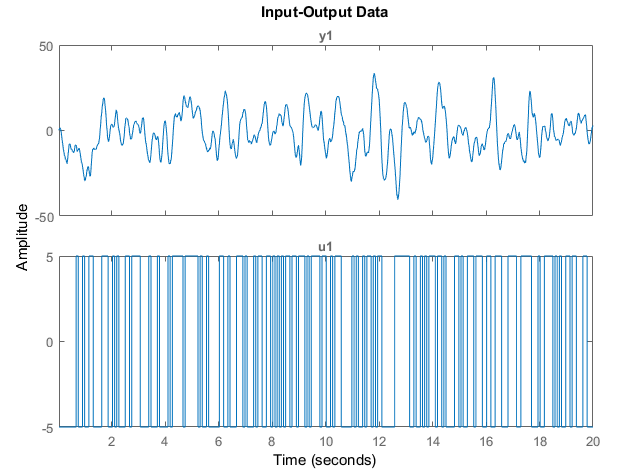
\includegraphics[width=0.5\textwidth]{Images/1.png}
\caption{ la simulation du système}
\end{figure}

Le script suivant est pour analyser la réponse fréquentielle du système, le SBPA, et la sortie:
\label{matlab}
\lstinputlisting[caption = {Le script pour analyser le système et les entrées et les sorties}]{3.m}
\subsubsection{degré de persistance}
Le degré de persistance du signale d'entrée (SBPA) est 50, que signifie que ce signale est riche en fréquences (au moins 50 fréquences distinctes), et ça nous permet d'identifier le système avec une grande précision parce que le signale permet d'obtenir un modèle avec 50 paramètres si on veut augmenter la précision.


\subsubsection{La réponse fréquentielle du système:}
La simulation du script en dessus, nous permet d'obtenir le résultat suivant:
\begin{figure}[H]
\centering
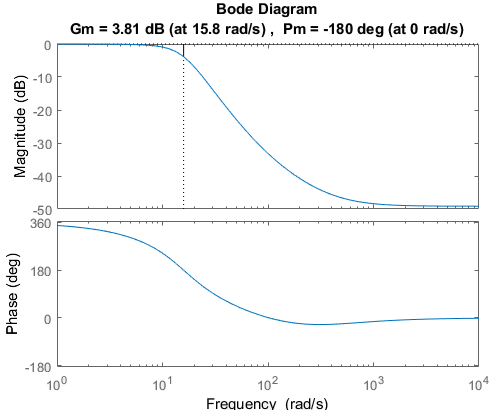
\includegraphics[width=0.5\textwidth]{Images/2.png}
\caption{ la réponse fréquentielle du système}
\end{figure}
\underline{Remarque:}\\
Le système ressemble á un filtre Passe Bas, avec une fréquence de coupure 15.8.

\subsubsection{Le spectre du signale d'entrée SBPA:}
\begin{figure}[H]
\centering
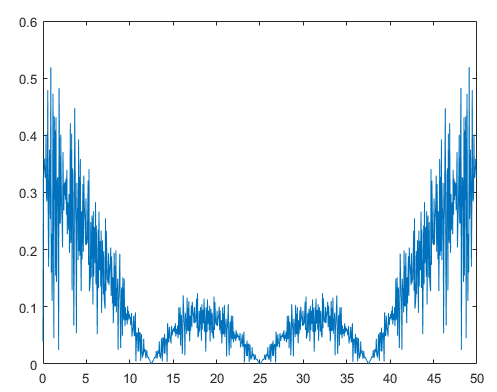
\includegraphics[width=0.5\textwidth]{Images/3.png}
\caption{ le spectre du SBPA}
\end{figure}
\underline{Remarque:}\\
Le signale est riche en fréquences et contient toutes les fréquences du système (la bande passante du système).

\subsubsection{Le spectre du signale de sortie:}
\begin{figure}[H]
\centering
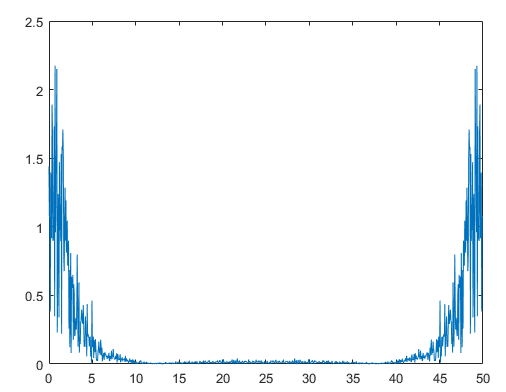
\includegraphics[width=0.5\textwidth]{Images/4.png}
\caption{ le spectre du signale de sortie}
\end{figure}
\underline{Remarque:}\\
La réponse fréquentielle du système explique bien ce résultat, en effet on voie que toutes les fréquence supérieur á 15 Hz sont rejeté, c'est l'effet que le système est un filtre passe bas á 15 Hz de fréquence de coupure.

Le degré de persistance du signale d'entrée (qui est 50), et le graph du spectre nous ont montré que le signale SBPA a été bien choisi pour exciter toutes les fréquences du système afin d'avoir une précision élevée du modèle identifié.
\newpage
\subsection{Identification du système}
On utilise plusieurs méthodes, et pour chaque méthode on utilise un algorithme qui cherche les ordres de modèle pour lesquels le FPE du système est optimal (le code qui est utilisé dans le TD pour cherché un FPE optimal).

\subsubsection{Moindres carrés ordinaires}
Le système maintenant est considéré comme ARX, et on a supposé qu'il n'y pas de bruit (malgré que le bruit exit sur le système á identifier).

\label{matlab}
\lstinputlisting[caption = {Le script Identifier le système par la méthode moindre carré}]{4.m}
La simulation nous donne le résultat suivants:
\begin{figure}[H]
\centering
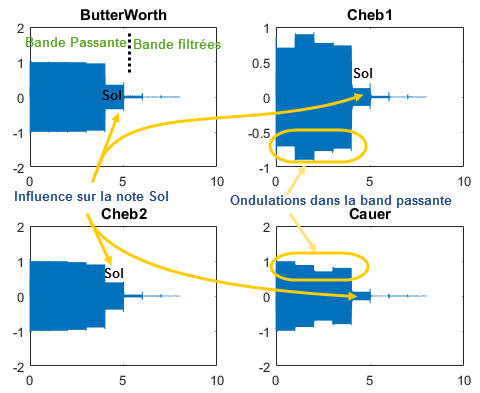
\includegraphics[width=0.5\textwidth]{Images/5.png}
\caption{ le modèle trouvé par le moindre carré}
\end{figure}

\underline{Remarque:}
Le degré pour lequel le FPE est otimale est : $na = 5$ , $nb=3$ ,et $nk=1$. 

\subsubsection{Variable instrumentale á quatre étages}
Le système maintenant est considéré comme ARX, mais en consédirant que le bruit cette fois ci. La méthode IV ajoute une variable instrumentale pour rejeter l'effet du bruit du système sur l'identification.

\label{matlab}
\lstinputlisting[caption = {Le script Identifier le système par la méthode de Variable instrumentale}]{5.m}
La simulation nous donne le résultat suivants:
\begin{figure}[H]
\centering
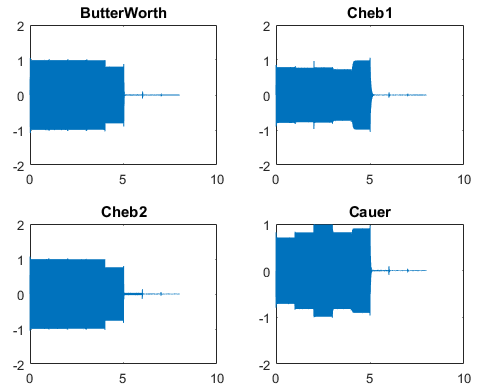
\includegraphics[width=0.5\textwidth]{Images/6.png}
\caption{ le modèle trouvé par la Variable instrumentale}
\end{figure}

\underline{Remarque:}
Le degré pour lequel le FPE est otimale est : $na = 2$ , $nb=4$ ,et $nk=1$. 

\subsubsection{Maximum de vraisemblance}
Le système maintenant est considéré comme ARMAX, et cette méthode va prendre en condédiraiton l'effet du bruit.
\label{matlab}
\lstinputlisting[caption = {Le script Identifier le système par la méthode Maximum de vraisemblance}]{6.m}
La simulation nous donne le résultat suivants:
\begin{figure}[H]
\centering
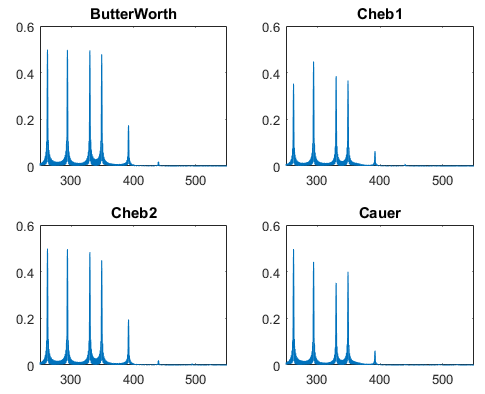
\includegraphics[width=0.5\textwidth]{Images/7.png}
\caption{ le modèle trouvé par Maximum de vraisemblance}
\end{figure}

\underline{Remarque:}
Le degré pour lequel le FPE est otimale est : $nb = 5$ , $nb=5$ ,et $nk=1$. 

\underline{Changement de paramètres pour améliorer l'identification:}
On utiliser ce scripte:
\label{matlab}
\lstinputlisting[caption = {Le script pour le changement de paramètres pour améliorer l'identification}]{7.m}

\underline{Remarque:}
Les résultats de simulation sont toujours les mêmes sauf pour l'option 'grad', qui donne des résultats non désirés.

\subsubsection{Méthode d'erreur de sortie}
Le script utilisé:
\label{matlab}
\lstinputlisting[caption = {Le script Identifier le système par la méthode Méthode d'erreur de sortie}]{8.m}
La simulation nous donne le résultat suivants:
\begin{figure}[H]
\centering
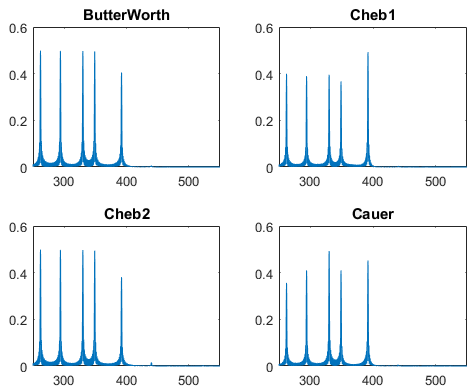
\includegraphics[width=0.5\textwidth]{Images/8.png}
\caption{ le modèle trouvé par Méthode d'erreur de sortie}
\end{figure}

\subsection{La fonction validation(modex,modid)}
Le script de cette fonction:
\label{matlab}
\lstinputlisting[caption = {Le script de la fonction validation(modex,modid)}]{9.m}

Le script suivant est pour comparer le modeles en utilisant la fonction 'validation':
\label{matlab}
\lstinputlisting[caption = {Le script de la fonction validation(modex,modid)}]{10.m}

La simulation donne les résultats suivants:
\subsection{Moindre carré}
\begin{figure}[H]
\centering
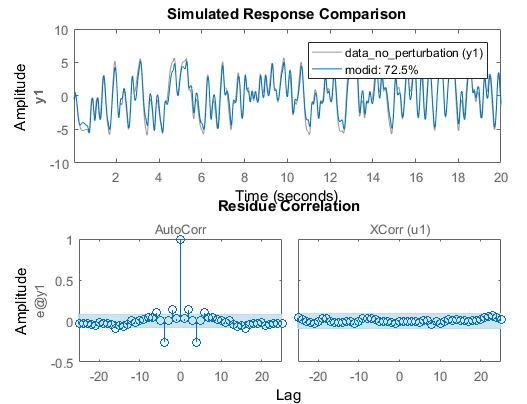
\includegraphics[width=0.5\textwidth]{Images/10.png}
\caption{ le modèle trouvé par Méthode d'erreur de sortie}
\end{figure}

\subsection{Méthode de variable instrumentale}
\begin{figure}[H]
\centering
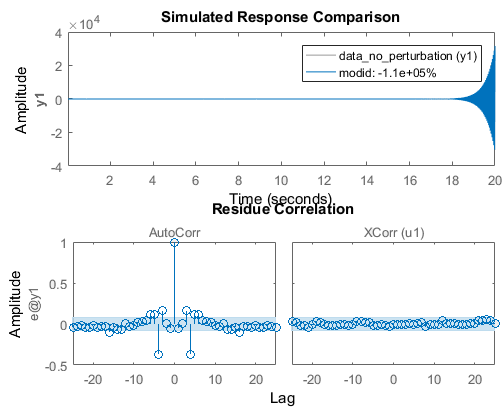
\includegraphics[width=0.5\textwidth]{Images/11.png}
\caption{ le modèle trouvé par Méthode d'erreur de sortie}
\end{figure}

\subsection{Méthode de maximum vraisemblance}
\begin{figure}[H]
\centering
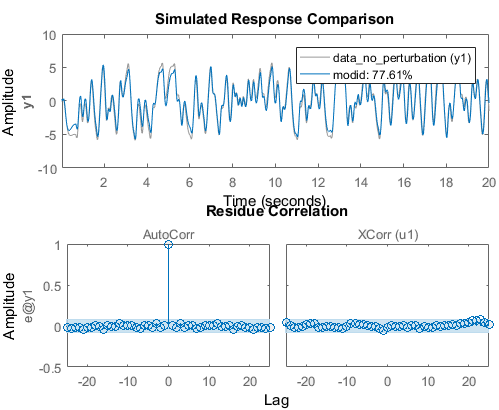
\includegraphics[width=0.5\textwidth]{Images/12.png}
\caption{ le modèle trouvé par Méthode d'erreur de sortie}
\end{figure}

\subsection{Méthode de l'erreur de sortie}
\begin{figure}[H]
\centering
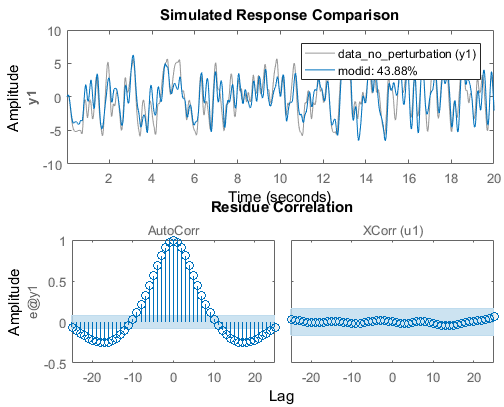
\includegraphics[width=0.5\textwidth]{Images/13.png}
\caption{ le modèle trouvé par Méthode d'erreur de sortie}
\end{figure}

\subsection{La fonction analyse(modex,modid)}
Le script de cette fonction:
\label{matlab}
\lstinputlisting[caption = {Le script de la fonction analyse(modex,modid)}]{11.m}


%77777777777777777777777777777777777777777777777777777777777777777777777777777777777
\section{Identification d'une maquette d'asservissement de position}
\subsection{Modélisation du processus}

\subsubsection{La fonction de transfert entre Z et la consigne}
Pour cela, on calcul la fonction de transfert entre Y et la consigne.
La fonction de transfert entre Y et U en boucle ouverte: $$G_0(s)=\frac{Y(s)}{U(s)} $$
En boucle fermée la fonction de transfert entre Y et la consigne est : $$ \frac{Y}{Y_c}=\frac{G_0.P}{1+G_0.P}$$
Par contre : $$ \frac{Z}{Y} = \frac{\frac{Z}{U}}{\frac{Y}{U}}=\frac{K_z.s}{K_y}$$
En on déduit que : $$ Z = \frac{K_z.s}{K_y}.Y = \frac{K_z.s}{K_y}.\frac{G_0.P}{1+G_0.P}.Y_c$$
Il résulte que: $$\frac{Z(s)}{Y_c(s)} = \frac{K_z.P.s}{s.(1+T_1.s).(1+T_2.s)+K_y.P}$$
Où bien:
$$\frac{Z(s)}{Y_c(s)} = \frac{K_z.P.s}{T_1.T_2.s^3+(T_1+T_2).s^2 + s +K_y.P}$$
$$\frac{Z(s)}{Y_c(s)} = \frac{b_1.s + b_0}{a_3.s^3 + a_2.s^2 + a_1.s + a_0}$$
telle que:\\

$$b_0 = 0$$  $$b_1 = K_z.P$$ $$a_0 = K_y.P$$ $$a_1 = 1$$ $$a_2 = T_1+T_2$$ $$a_3 = T_1.T_2$$


\subsubsection{La forme de la fonction de transfert discréte entre Z et la consigne}
Si on utilise la transformation bilinéaire: $$ s = \frac{2}{T_e}\frac{1-z^{-1}}{1+z^{-1}}$$ 
On obtient une fonction dont la forme est 
$$F(z) = \frac{b_1.\frac{2}{T_e}\frac{1-z^{-1}}{1+z^{-1}}}{a_3.(\frac{2}{T_e}\frac{1-z^{-1}}{1+z^{-1}})^3 + a_2.(\frac{2}{T_e}\frac{1-z^{-1}}{1+z^{-1}})^2 + a_1.(\frac{2}{T_e}\frac{1-z^{-1}}{1+z^{-1}}) + a_0}$$
En multipliant le numérateur et dénominateur par $(1+z^{-1})^3$ on obtient un fonction dont les degrés de numérateur et dénominateur égalent á 3:
$$ F_z = \frac{\beta_0 + \beta_1.z^{-1}+\beta_2.z^{-2}+\beta_3.z^{-3}}{\alpha_0 + \alpha_1.z^{-1}+ \alpha_2.z^{-2}+ \alpha_3.z^{-3}}$$

\subsubsection{Identification du processus}

\subsubsection{Les paramètres de la fonction de transfert}
On a montré que:
$$\frac{Z(s)}{Y_c(s)} = \frac{b_1.s + b_0}{a_3.s^3 + a_2.s^2 + a_1.s + a_0}$$
telle que:\\
$$b_0 = 0$$  $$b_1 = K_z.P$$ $$a_0 = K_y.P$$ $$a_1 = 1$$ $$a_2 = T_1+T_2$$ $$a_3 = T_1.T_2$$
\subsubsection{Identification en utilisant la fonction de transfert discrète}
si on suppose qu'on utilise un bloqueur d'ordre 0 alors:
$$F_z = \frac{Z(z)}{Y_c(z)} = ((1-z^{-1})TZ(\frac{Z(s)}{Y_c(s).s})$$

La fréquence d'échantillonnage est de $1kHz$, que signifie que la période est $Te = \frac{1}{1000}$;
Le script suivant est pour charger les données de l'expérimentation dans un objet de 'data':
\label{matlab}
\lstinputlisting[caption = {Le script pour charger et simuler les données de l'expérimentation}]{11.m}

La simulation donne:
\begin{figure}[H]
\centering
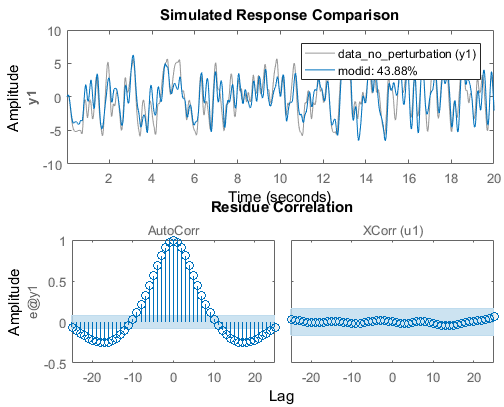
\includegraphics[width=0.5\textwidth]{Images/13.png}
\caption{ Simulation les donnée de l'expérience}
\end{figure}

L'entrée est un signale carrée périodique.

Le script suivant est pour utiliser la méthode de l'erreur de sortie pour identifier le système:
\label{matlab}
\lstinputlisting[caption = {Le script pour identifier le système}]{12.m}

Le résultat de compilation donne:
$$ F(s) = \frac{-0.01831 s^3 - 17.44 s^2 + 1.498e04 s + 1536}{s^3 + 605.7 s^2 + 3.684e04 s + 2.818e06} $$

On remarque que dans le numérateur, les termes multipliés par $s^3$,$s^2$, et $s^0$ sont trais négligeable par rapport á celui multiplié par $s$, donc on peut prendre :
$$ F(s) = \frac{1.498e04 s}{s^3 + 605.7 s^2 + 3.684e04 s + 2.818e06} $$
en devisant le numérateur et le dénomératuer par $3.684e04$ on obitient:
$$F(s)=\frac{0.4066 s}{  2.714e-05 s^3 + 0.01644 s^2 + s + 76.49}$$
D'où 
$$b_1 = K_z.P = 0.4066$$ $$a_0 = K_y.P =  76.49$$ $$a_1 = 1$$ $$a_2 = T_1+T_2 = 0.01644$$ $$a_3 = T_1.T_2 =2.714e-05$$
On en déduit que:
$$K_z = b1 / P = 0.1402$$
$$K_y = a0/P =26.3769 $$
$$T_1 = (a2+\sqrt{a2^2-4*a3})/2 = 0.0146$$
$$T_2 = a2-T1 = 0.0019$$

Le script suivant est pour calculer F(s) et la valider:
\label{matlab}
\lstinputlisting[caption = {Le script pour calculer F(s) et la simuler}]{13.m}

\subsubsection{Validation}
si on compare la la fonction $F(s)$ avec les données de l'expérimentation on trouve un $FIT=90.21\%$, comme la figure montre:

\begin{figure}[H]
\centering
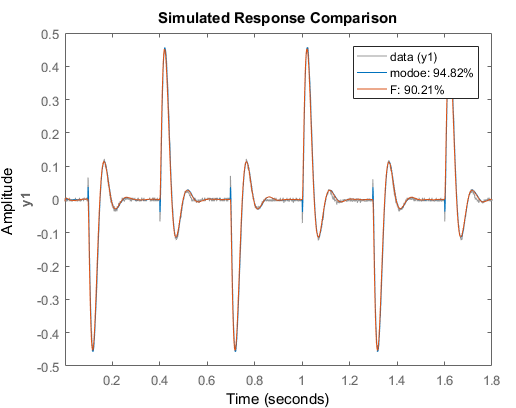
\includegraphics[width=0.5\textwidth]{Images/15.png}
\caption{ Comparaison}
\end{figure}

\underline{Remarque}
	L'identification est assez précise que le $FIT=90.21\%$

\subsection{Identification direct en utilisant }
Le script pour identifier directement le systeme:
\label{matlab}
\lstinputlisting {14.m}

  
  De la même façon on trouve que:
  $$F(s)=\frac{7524 s + 228.2 }{s^3 + 312 s^2 + 2.068e04 s + 1.383e06}$$ $$\simeq \frac{ 0.3638 s}{4.836e-05 s^3 + 0.01509 s^2 + s + 66.88} $$
  Et on en déduit les paramètres physiques:
$$K_z = b1 / P = 0.1255$$
$$K_y = a0/P =23.0608 $$
$$T_1 = (a2+\sqrt{a2^2-4*a3})/2 = 0.0105$$
$$T_2 = a2-T1 = 0.0046$$
  \subsubsection{Validation}
  L'identification est assez précise (surtout pour la commande):

\begin{figure}[H]
\centering
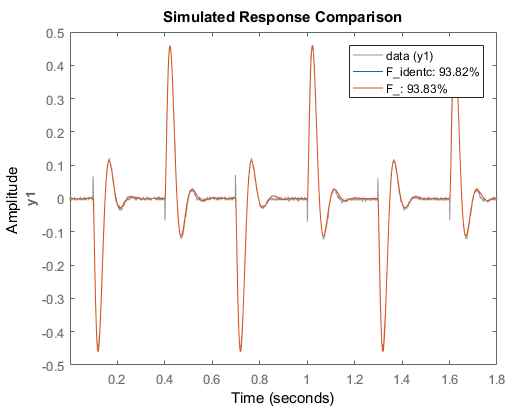
\includegraphics[width=0.5\textwidth]{Images/16.png}
\caption{Comparaison}
\end{figure}

\subsection{Identification direct en utilisant la fonction idgrey et pem}
On a la fonction de transfert est de la forme suivante:
$$F(s)=\frac{Z(s)}{Y_c(s)} = \frac{b_1.s}{a_3.s^3 + a_2.s^2 + a_1.s + a_0}$$ 
$$ = \frac{\frac{K_z.P}{T_1.T_2} s}{s^3 + \frac{T_1+T_2}{T_1.T_2}s^2 + \frac{1}{T_1.T_2}s + \frac{K_y.P}{T_1.T_2}}$$ 
$$ = \frac{\beta_1.s}{s^3 + \alpha1.s^2 + \alpha2.s + \alpha3}$$ 

Si on prend $x_3 = Z$ , $x_2 = \dot Z$, et $x_1 = \ddot Z$ 
on obtient la forme canonique suivante:
%\dot X = 

\begin{equation}
\dot{X}=
\begin{pmatrix}  -\alpha_1 & -\alpha_2 & -\alpha_3 \\ 1 & 0 & 0\\ 0 & 1 & 0 \end{pmatrix}X
+\begin{pmatrix} 1 \\ 0 \\ 0 \end{pmatrix} Y_c \\
\end{equation}

\begin{equation}
Z  = \begin{pmatrix} 0 \\ b_1 \\ 0 \end{pmatrix}X
\end{equation}

Le script pour la fonction idgrey :
\label{matlab}
\lstinputlisting {15.m}

Le script pour l'identification:
\label{matlab}
\lstinputlisting {16.m}

Le résultat de simulation:\\

Fit to estimation data: $94.02\%$ \\             
FPE: $6.008e-05$, MSE: $5.981e-05$\\\\


La comparaison avec les données 'data':

\begin{figure}[H]
\centering
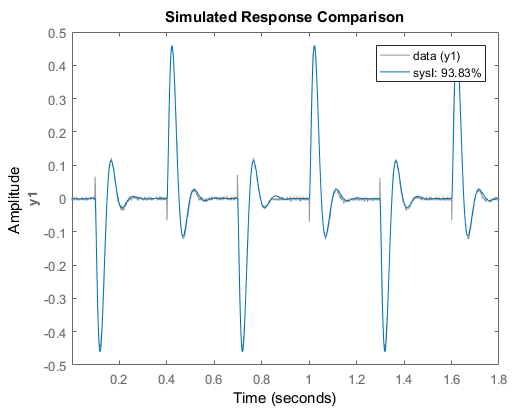
\includegraphics[width=0.5\textwidth]{Images/17.png}
\caption{Comparaison}
\end{figure}

La fonction 
$$F(s)=\frac{8400 s}{s^3 + 350 s^2 + 2.253e04 s + 1.549e06} $$
Les valeurs estimées des paramètres:
$$K_z = b1 / P = 0.1286$$
$$K_y = a0/P =23.7079 $$
$$T_1 = (a2+\sqrt{a2^2-4*a3})/2 =0.0118$$
$$T_2 = a2-T1 =  0.0038$$


\section{Identification d'un système acoustique}


\subsection{découplage de données en trois parties}

\label{matlab}
\lstinputlisting {17.m}

présentation des trois morceaux en même plan:

\begin{figure}[H]
\centering
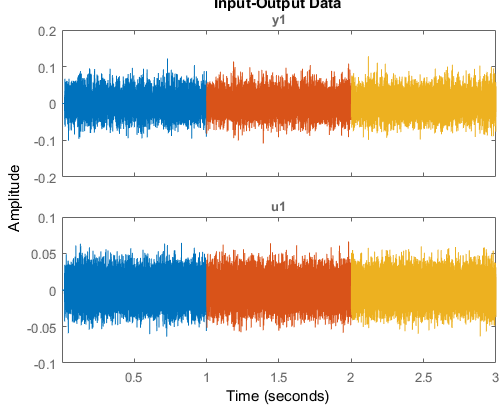
\includegraphics[width=0.5\textwidth]{Images/18.png}
\caption{Comparaison}
\end{figure}

\subsection{identification le modèles á temps discret á partir de chaque jeu de données}
On a utilisé un algorithm pour trouvé le meilleur ordre qui optimise le critère FPE, 
Le script Matlab pour le suivant:
\label{matlab}
\lstinputlisting {18.m}

\subsection{Validation croisée:}
On compare chaque modèle avec les autres domaines restants qu'on a utilisé pour identifier les autres deux modèles:
\label{matlab}
\lstinputlisting {19.m}

Le résultat de simulation:
\begin{figure}[H]
\centering
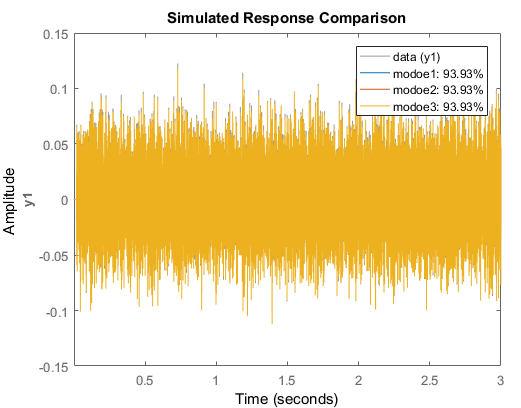
\includegraphics[width=0.5\textwidth]{Images/19.png}
\caption{Comparaison entre les trois modèles et les données de l'expérience}
\end{figure}

Les trois modèles sont de même précision et sont tous assez précis.
\subsection{La réponse impulsionnelle}

\label{matlab}
\lstinputlisting {20.m}
Le résultat de simulation:

\begin{figure}[H]
\centering
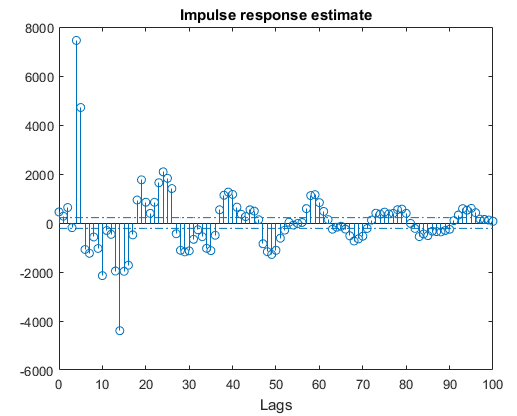
\includegraphics[width=0.5\textwidth]{Images/20.png}
\caption{La réponse impulsionnelle}
\end{figure}

\underline{Remarque}
On peut dire que le retard est de 4 ou 3 unités .

\subsection{Identification pour plusieurs ordres de modèles}
Le script Matlab:
\label{matlab}
\lstinputlisting {21.m}

Le résultat de simulation:
\begin{figure}[H]
\centering
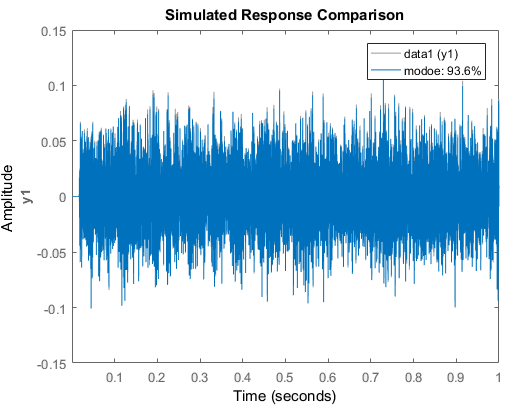
\includegraphics[width=0.5\textwidth]{Images/21.png}
\caption{Comparaison entre le modèle et les données de l'expérience}
\end{figure}

Le modèles est assez précis.



\end{document}

